% !TeX program = lualatex
% !TeX encoding = utf8
% !TeX spellcheck = uk_UA
% !BIB program = bibtex8

\documentclass[14pt]{extarticle}
	\usepackage{polyglossia}
	\setmainlanguage{ukrainian}
	\setotherlanguages{english, russian}
	\setsansfont{CMU Sans Serif}
	\setmainfont[Ligatures=TeX]{CMU Serif}
	\setmonofont{Consolas}
	\usepackage{minted, xcolor}
	\definecolor{lightgray}{gray}{0.99}
	\renewcommand\listoflistingscaption{List of source codes}
	\renewcommand\theFancyVerbLine{\scriptsize\arabic{FancyVerbLine}}
	%------------------------------------------------------------------
	\RequirePackage[%
	a4paper,%
	footskip=1cm,%
	headsep=0.3cm,% 
	top=2cm, %поле сверху
	bottom=2cm, %поле снизу
	left=2cm, %поле ліворуч
	right=2cm, %поле праворуч
	]{geometry}
	%-------------Подавление висячих строк--------------------------------
	\clubpenalty =10000
	\widowpenalty=10000
	%-------------Інтервали-----------------------------------------------
	\setlength{\parskip}{0.5ex}%
	\setlength{\parindent}{2.5em}%
	\renewcommand{\baselinestretch}{1.1}
	%---------------------------------------------------------------------
    \usepackage{graphicx}
\title{Фігури Ліссажу\\ Реалізація за допомогою \texttt{Python}}
\date{}
\begin{document}
\maketitle

\section{Що таке фігури Ліссажу?}

Фігури Ліссажу -- замкнуті траєкторії, які прокреслюються точкою, що здійснює одночасно два гармонійних коливання у двох взаємно перпендикулярних напрямках. Вперше вивчені французьким науковцем Ж. Ліссажу (фр. J. Lissajous; 1822—1880). Вид фігур залежить від співвідношення між періодами (частотами), фазами і амплітудами обох коливань. У найпростішому випадку (за рівності обох періодів) фігури являють собою еліпси, які при різниці фаз 0 або π вироджуються у відрізки прямих, а при різниці фаз π/2 і рівності амплітуд перетворюються в коло. Якщо періоди обох коливань не точно збігаються, то різниця фаз весь час змінюється, внаслідок чого еліпс весь час деформується. При істотно різних періодах фігури Ліссажу не спостерігаються, оскільки еліпс деформується швидко, картина розмивається. Однак, якщо періоди відносяться як цілі числа, то через проміжок часу, рівний найменшому кратному обох періодів, точка, що рухається, знову повертається в те ж положення — виходять фігури Ліссажу складнішої форми. Фігури Ліссажу вписуються в прямокутник, центр якого збігається з початком координат, а сторони паралельні осям координат і розташовані по обидва боки від них на відстанях, рівних амплітудами коливань. При цьому кількість дотиків фігури до сторін прямокутника, в який вона вписана дає відношення періодів двох коливань.

\section{Реалізація алгоритму}

\begin{center}
    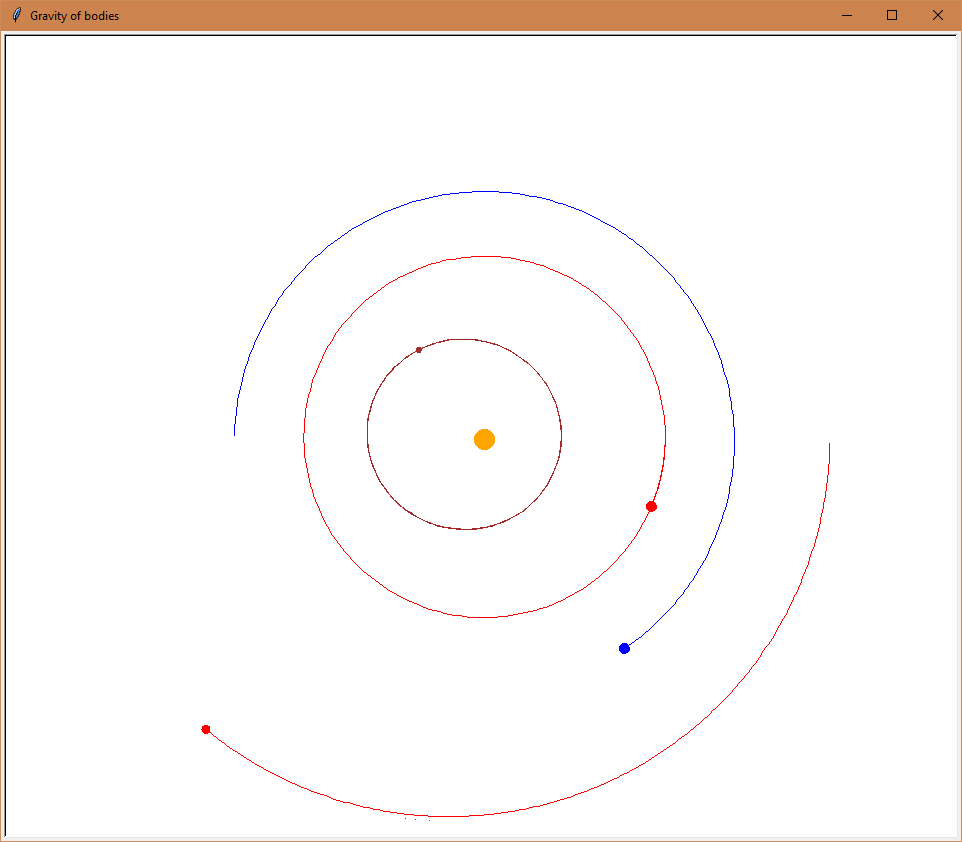
\includegraphics[width=\linewidth]{Pic1}
\end{center}

\begin{minted}
[
frame=lines,
framesep=2mm,
baselinestretch=1.2,
bgcolor=lightgray,
fontsize=\footnotesize,
linenos,
breaklines
]
{python}
# -*- coding: utf-8 -*-

from turtle import Turtle, Screen
from math import pi, cos
from timeit import default_timer as timer

# %% class
class Body(Turtle):
     """
     Oscilating bodies.
     Amplitude - Object Amplitude
     omega     - Object Angular Velocity
     phi       - Phase Shift
     k1        - x Coordinate Angular Velocity amplifier
     k2        - y Coordinate Angular Velocity amplifier
     """
     def __init__(self, Amplitude = 100, omega = 1, k1 = 1, k2 = 1, phi = pi/2):
        Turtle.__init__(self)
        self.Amplitude = Amplitude
        self.omega = omega
        self.k1 = k1
        self.k2 = k2
        self.phi  = phi

timer_t = Turtle(visible=False)
timer_t.penup()
timer_t.setposition(300,300)

global screen
screen = Screen()
screen.tracer(0)

# %% loop function
def loop(bodies):
    """
    The movement of bodies in accordance with a sinusoidal law
    """ 
    for body in bodies: 
        body.penup()
        body.showturtle()
        body.shape('circle')
        body.speed(1)

    t0 = timer() # strange nonzeroth starting value of time
    while True:
        time =  timer() - t0
        for body in bodies:
            body.x = body.Amplitude * cos(body.k1*body.omega * time)            # x Coordinate law of motion
            body.y = body.Amplitude * cos(body.k2*body.omega * time - body.phi) # y Coordinate law of motion
            body.goto(body.x, body.y)
            body.pendown()


        timer_t.write('t = ' + str(round(time, 2)))
        screen.update()
        timer_t.undo()

# %% Axis Draw

def AxisDraw(axis, maxval):
    """
    Drawing Cartesian coordinates
    """
    axis.speed(0)
    axis.setposition(0,-maxval)
    axis.goto(0,maxval)
    axis.penup()
    axis.setposition(-maxval,0)
    axis.pendown()
    axis.goto(maxval,0)

# %% Main fumnction

def main():
    global screen
    screen = Screen()
    axis = Turtle(visible=False)
    AxisDraw(axis, 300)

    body1 = Body(Amplitude=200, omega=1, k1=1, k2=2, phi=0)
    body1.color('red')

    body2 = Body(Amplitude=200, omega=1, k1=1, k2=2, phi=pi/2)
    body2.color('blue')

    loop([body1, body2])

if __name__ == '__main__':
    main()
    screen.mainloop()
\end{minted}
\end{document}